\documentclass[10pt, compress]{beamer}

\usetheme{m}

\usepackage{booktabs}
\usepackage[scale=2]{ccicons}
\usepackage{minted}
\usepackage{wrapfig}

\usemintedstyle{trac}

\title{}
\subtitle{On Statistical Properties of\\Arbiter Physical Unclonable Function}
\date{\today}
\author{Phillip Gajland}
\institute{KTH Royal Institute of Technology}

\begin{document}

\begin{frame}[plain,t]
    
    \begin{wrapfigure}{r}{0.2\textwidth}
        \begin{flushright}
        \vspace{-2.25cm}
        
\includegraphics[width = 20mm]{figures/kth_logo.png}
        \end{flushright}
    \end{wrapfigure}
    
    \vspace{2cm}
    
    {\large\textbf{On Statistical Properties of\\[0.25cm]
    Arbiter Physical Unclonable Functions}}
    \\\rule{7.5cm}{1pt}
    
    \vspace{0.25cm}
    
    {\large\textbf{Phillip Gajland}}
    
    \vspace{0.5cm}
    
    \begin{wrapfigure}{r}{0.3\textwidth}
        \begin{flushright}
        \vspace{-1cm}
        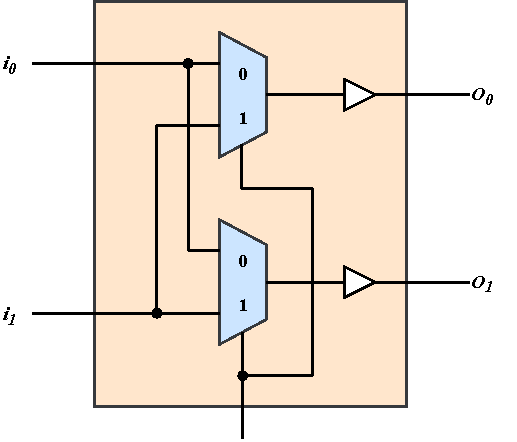
\includegraphics[width = 40mm]{figures/switch_block_detailed.pdf}
        \end{flushright}
    \end{wrapfigure}
    
    {\normalsize
    \begin{tabular}{ r l }
    Examiner: & Prof. Dr. Elena Dubrova\\
    Supervisor: & Dr. Felipe Marranghello
    \end{tabular}}
    
    \vspace{1cm}
    
    \textbf{May 28\textsuperscript{th} 2018}

\end{frame}

\begin{frame}{Content}
    \tableofcontents
\end{frame}

\begin{frame}{Problem}
    \begin{itemize}
        \item unique device identifiers
        \item secure key storage
        \item intelectual property theft
        \item Xilinx Zynq Ultrascale+ 
        \item Altera Stratix 10 FPGAs
    \end{itemize}
\end{frame}



\begin{frame}{Boolean Functions}
    
\end{frame}


\begin{frame}{Physical Unclonable Functions}
    
\end{frame}

\section{Abiter PUFs}

\begin{frame}{switch block}
    \begin{figure}
        \centering
        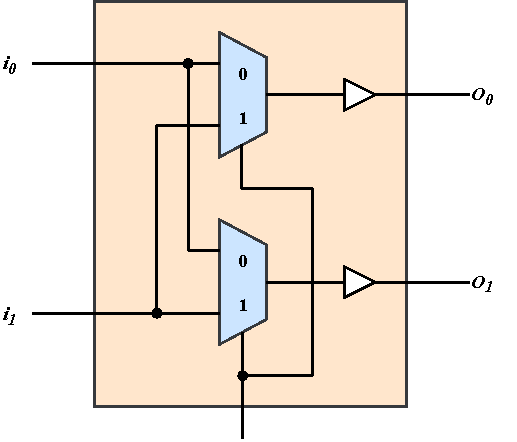
\includegraphics[width=0.6\textwidth]{figures/switch_block_detailed.pdf}
        \caption{Schematic of a switch block}
    \end{figure}
\end{frame}


\begin{frame}{Abiter PUFs}
    \begin{figure}[ht]
        \centering
        \begin{subfigure}[b]{0.58\textwidth}
            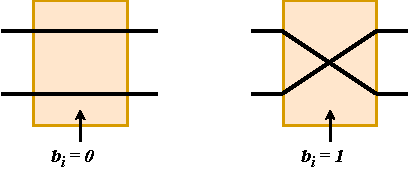
\includegraphics[width=\textwidth]{figures/switch_block_operations.pdf}
            \label{fig:switch_block_operations}
        \end{subfigure}
        \begin{subfigure}[b]{0.33\textwidth}
            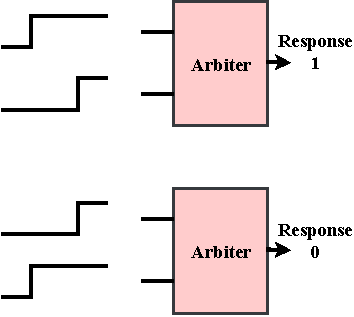
\includegraphics[width=\textwidth]{figures/arbiter_operation.pdf}
            \label{fig:arbiter_operations}
        \end{subfigure}
        \caption{Arbiter PUF operations}\label{fig:puf_operations}
    \end{figure}
\end{frame}


\begin{frame}{Abiter PUFs}
    \begin{figure}
        \centering
        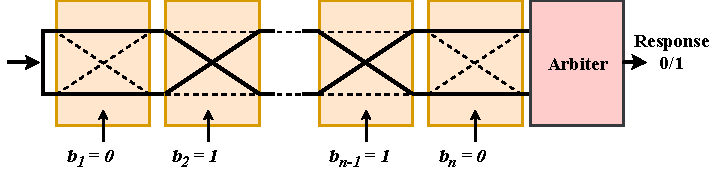
\includegraphics[width=\textwidth]{figures/multiple_switch_blocks.pdf}
        \caption{Multiple switch blocks in series form a PUF}
    \end{figure}
\end{frame}

\begin{frame}{Previous Studies}
	\begin{itemize}
		\item Machine Learning attacks
        \item Stability
	\end{itemize}
\end{frame}


\begin{frame}{Functions}
    \begin{figure}
        \centering
        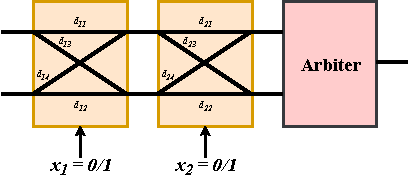
\includegraphics[width=0.8\textwidth]{figures/2_switch_blocks_paths.pdf}
        \caption{Arbiter PUF paths}
    \end{figure}
\end{frame}


\begin{frame}{table}

  \begin{table}[ht]
    \centering
    \caption{4 Boolean functions induced by an arbiter PUF with one switch block.}
    \def\arraystretch{1.2}
    $\begin{tabu}{c|c|c|c}
         \cline{2-3}
         & \multicolumn{2}{c|}{\text{Challenge}}                      &                                        \\ \cline{2-4}
                                  & x_1 = 0         & x_1 = 1         & \multicolumn{1}{||c|}{f(x_1)}          \\ \hline \tabucline[2pt]{-}
         \multicolumn{1}{|c|}{00} & d_{11} < d_{12} & d_{13} > d_{14} & \multicolumn{1}{||c|}{0}               \\ \hline
         \multicolumn{1}{|c|}{01} & d_{11} < d_{12} & d_{13} < d_{14} & \multicolumn{1}{||c|}{1}               \\ \hline
         \multicolumn{1}{|c|}{10} & d_{11} > d_{12} & d_{13} < d_{14} & \multicolumn{1}{||c|}{x_1}             \\ \hline
         \multicolumn{1}{|c|}{11} & d_{11} > d_{12} & d_{13} > d_{14} & \multicolumn{1}{||c|}{\overline{x_1}}  \\ \hline
    \end{tabu}$
\end{table}
  
\end{frame}


\begin{frame}{table}

    \begin{center}
        Deltas instead of absolute values
    \end{center}
    \[ \Delta_{mj-nk} = d_{mj} - d_{nk} \]

\end{frame}


\begin{frame}{table}

  \begin{table}[ht]
    \def\arraystretch{1.3}
    $\begin{tabu}{c|c|c|c}
         \cline{2-3}
         & \multicolumn{2}{c|}{\text{Challenge}}                            &                                        \\ \cline{2-4}
                                  & x_1 = 0            & x_1 = 1            & \multicolumn{1}{||c|}{f(x_1)}          \\ \hline \tabucline[2pt]{-}
         \multicolumn{1}{|c|}{00} & \Delta_{11-12} < 0 & \Delta_{13-14} > 0 & \multicolumn{1}{||c|}{0}               \\ \hline
         \multicolumn{1}{|c|}{01} & \Delta_{11-12} < 0 & \Delta_{13-14} < 0 & \multicolumn{1}{||c|}{1}               \\ \hline
         \multicolumn{1}{|c|}{10} & \Delta_{11-12} > 0 & \Delta_{13-14} < 0 & \multicolumn{1}{||c|}{x_1}             \\ \hline
         \multicolumn{1}{|c|}{11} & \Delta_{11-12} > 0 & \Delta_{13-14} > 0 & \multicolumn{1}{||c|}{\overline{x_1}}  \\ \hline
    \end{tabu}$
\end{table}
  
\end{frame}


\begin{frame}[fragile]
  \frametitle{truth table}
  
  \begin{table}[ht]
    \centering
    \label{truth_table_2_bit}
  \def\arraystretch{1.2}
  \resizebox{\linewidth}{!}{  
    $\begin{tabu}{c|c|c|c|c|c}
        \cline{2-5}
        & \multicolumn{4}{c|}{\text{Challenge}}                        &                                                                                                                                                               \\ \cline{2-6}
                                   & x_2 x_1 = 0 0                     & x_2 x_1 = 0 1                     & x_2 x_1 = 1 0                     & x_2 x_1 = 1 1                     & \multicolumn{1}{||c|}{f(x_1, x_2)}                \\ \tabucline[2pt]{-}
        \multicolumn{1}{|c|}{0000} & d_{11} + d_{21} < d_{12} + d_{22} & d_{14} + d_{21} < d_{13} + d_{22} & d_{12} + d_{24} < d_{11} + d_{23} & d_{13} + d_{24} < d_{14} + d_{23} & \multicolumn{1}{||c|}{0}                          \\ \hline
        \multicolumn{1}{|c|}{0001} & d_{11} + d_{21} < d_{12} + d_{22} & d_{14} + d_{21} < d_{13} + d_{22} & d_{12} + d_{24} < d_{11} + d_{23} & d_{13} + d_{24} > d_{14} + d_{23} & \multicolumn{1}{||c|}{x_1 x_2}                    \\ \hline
        \multicolumn{1}{|c|}{0010} & d_{11} + d_{21} < d_{12} + d_{22} & d_{14} + d_{21} < d_{13} + d_{22} & d_{12} + d_{24} > d_{11} + d_{23} & d_{13} + d_{24} < d_{14} + d_{23} & \multicolumn{1}{||c|}{\overline{x_1} x_2}         \\ \hline
        \multicolumn{1}{|c|}{0011} & d_{11} + d_{21} < d_{12} + d_{22} & d_{14} + d_{21} < d_{13} + d_{22} & d_{12} + d_{24} > d_{11} + d_{23} & d_{13} + d_{24} > d_{14} + d_{23} & \multicolumn{1}{||c|}{x_2}                        \\ \hline
        \multicolumn{1}{|c|}{0100} & d_{11} + d_{21} < d_{12} + d_{22} & d_{14} + d_{21} > d_{13} + d_{22} & d_{12} + d_{24} < d_{11} + d_{23} & d_{13} + d_{24} < d_{14} + d_{23} & \multicolumn{1}{||c|}{x_1 \overline{x_2}}         \\ \hline
        \multicolumn{1}{|>{\columncolor[gray]{.8}}c|}{0101} & d_{11} + d_{21} < d_{12} + d_{22} & d_{14} + d_{21} > d_{13} + d_{22} & d_{12} + d_{24} < d_{11} + d_{23} & d_{13} + d_{24} > d_{14} + d_{23} & \multicolumn{1}{||>{\columncolor[gray]{.8}}c|}{x_1}                        \\ \hline
        \multicolumn{1}{|c|}{0110} & d_{11} + d_{21} < d_{12} + d_{22} & d_{14} + d_{21} > d_{13} + d_{22} & d_{12} + d_{24} > d_{11} + d_{23} & d_{13} + d_{24} < d_{14} + d_{23} & \multicolumn{1}{||c|}{x_1 \xor x_2}               \\ \hline
        \multicolumn{1}{|c|}{0111} & d_{11} + d_{21} < d_{12} + d_{22} & d_{14} + d_{21} > d_{13} + d_{22} & d_{12} + d_{24} > d_{11} + d_{23} & d_{13} + d_{24} > d_{14} + d_{23} & \multicolumn{1}{||c|}{x_1 + x_2}                  \\ \hline
        \multicolumn{1}{|c|}{1000} & d_{11} + d_{21} > d_{12} + d_{22} & d_{14} + d_{21} < d_{13} + d_{22} & d_{12} + d_{24} < d_{11} + d_{23} & d_{13} + d_{24} < d_{14} + d_{23} & \multicolumn{1}{||c|}{\overline{x_1 + x_2}}       \\ \hline
        \multicolumn{1}{|c|}{1001} & d_{11} + d_{21} > d_{12} + d_{22} & d_{14} + d_{21} < d_{13} + d_{22} & d_{12} + d_{24} < d_{11} + d_{23} & d_{13} + d_{24} > d_{14} + d_{23} & \multicolumn{1}{||c|}{\overline{x_1 \xor x_2}}    \\ \hline
        \multicolumn{1}{|>{\columncolor[gray]{.8}}c|}{1010} & d_{11} + d_{21} > d_{12} + d_{22} & d_{14} + d_{21} < d_{13} + d_{22} & d_{12} + d_{24} > d_{11} + d_{23} & d_{13} + d_{24} < d_{14} + d_{23} & \multicolumn{1}{||>{\columncolor[gray]{.8}}c|}{\overline{x_1}}             \\ \hline
        \multicolumn{1}{|c|}{1011} & d_{11} + d_{21} > d_{12} + d_{22} & d_{14} + d_{21} < d_{13} + d_{22} & d_{12} + d_{24} > d_{11} + d_{23} & d_{13} + d_{24} > d_{14} + d_{23} & \multicolumn{1}{||c|}{\overline{x_1} + x_2}       \\ \hline
        \multicolumn{1}{|c|}{1100} & d_{11} + d_{21} > d_{12} + d_{22} & d_{14} + d_{21} > d_{13} + d_{22} & d_{12} + d_{24} < d_{11} + d_{23} & d_{13} + d_{24} < d_{14} + d_{23} & \multicolumn{1}{||c|}{\overline{x_2}}             \\ \hline
        \multicolumn{1}{|c|}{1101} & d_{11} + d_{21} > d_{12} + d_{22} & d_{14} + d_{21} > d_{13} + d_{22} & d_{12} + d_{24} < d_{11} + d_{23} & d_{13} + d_{24} > d_{14} + d_{23} & \multicolumn{1}{||c|}{x_1 + \overline{x_2}}       \\ \hline
        \multicolumn{1}{|c|}{1110} & d_{11} + d_{21} > d_{12} + d_{22} & d_{14} + d_{21} > d_{13} + d_{22} & d_{12} + d_{24} > d_{11} + d_{23} & d_{13} + d_{24} < d_{14} + d_{23} & \multicolumn{1}{||c|}{\overline{x_1x_2}}          \\ \hline
        \multicolumn{1}{|c|}{1111} & d_{11} + d_{21} > d_{12} + d_{22} & d_{14} + d_{21} > d_{13} + d_{22} & d_{12} + d_{24} > d_{11} + d_{23} & d_{13} + d_{24} > d_{14} + d_{23} & \multicolumn{1}{||c|}{1}                          \\ \hline
    \end{tabu}$ 
    }
\end{table}
  
\end{frame}


\begin{frame}{proof of conflict}
    \begin{tabular}{c c c}
        $\begin{cases} 
        d_{11} + d_{21} < d_{12} + d_{22}\\
        d_{14} + d_{21} > d_{13} + d_{22}\\
        d_{12} + d_{24} < d_{11} + d_{23}\\
        d_{13} + d_{24} > d_{14} + d_{23}
        \end{cases}$ 
        & $\implies$ &
        $\begin{cases} 
        &\Delta_{11-12} < -\Delta_{21-22}\\
        &\Delta_{21-22} > \Delta_{13-14}\\
        -&\Delta_{11-12} < \Delta_{23-24}\\
        &\Delta_{13-14} > \Delta_{23-24}
        \end{cases}$
    \end{tabular}
\end{frame}

\begin{frame}{proof of conflict}
    \begin{align*}
        -\Delta_{11-12} &< \Delta_{23-24} \text{ and } \Delta_{13-14} > \Delta_{23-24}\\
        -\Delta_{11-12} &< \Delta_{23-24} < \Delta_{13-14}\\
        -\Delta_{11-12} &< \Delta_{13-14}
    \end{align*}
    \begin{align*}
        \Delta_{11-12} &< -\Delta_{21-22} \text{ and } \Delta_{21-22} > \Delta_{13-14}\\
        -\Delta_{11-12} &> \Delta_{21-22} \text{ and } \Delta_{21-22} > \Delta_{13-14}\\
        \Delta_{13-14} &< \Delta_{21-22} < -\Delta_{11-12}\\
        \Delta_{13-14} &< -\Delta_{11-12}
    \end{align*}
    
    \begin{equation} \label{eqation}
        -\Delta_{11-12} < \Delta_{13-14} \neq \Delta_{13-14} < -\Delta_{11-12}
    \end{equation}
\end{frame}


% remove deltas no need - no need for working
% how can we solve this problem?
% introduce xor pufs
% how is the simulation done?
% explain the process of the simulation
% conclusion we show the distribution is not uniform 
% potential weekness, xoring can improve it.



\section{Results}

% ----------
% SINGLE PUF
% ----------

\begin{frame}{results}
    \begin{figure}
        \centering
        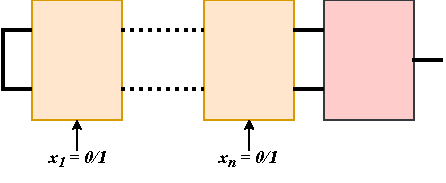
\includegraphics[width=0.7\textwidth]{figures/puf_1.pdf}
        \caption{Single Arbiter PUF}
    \end{figure}
\end{frame}

\begin{frame}{single arbiter puf}
    \begin{figure}
        \centering
        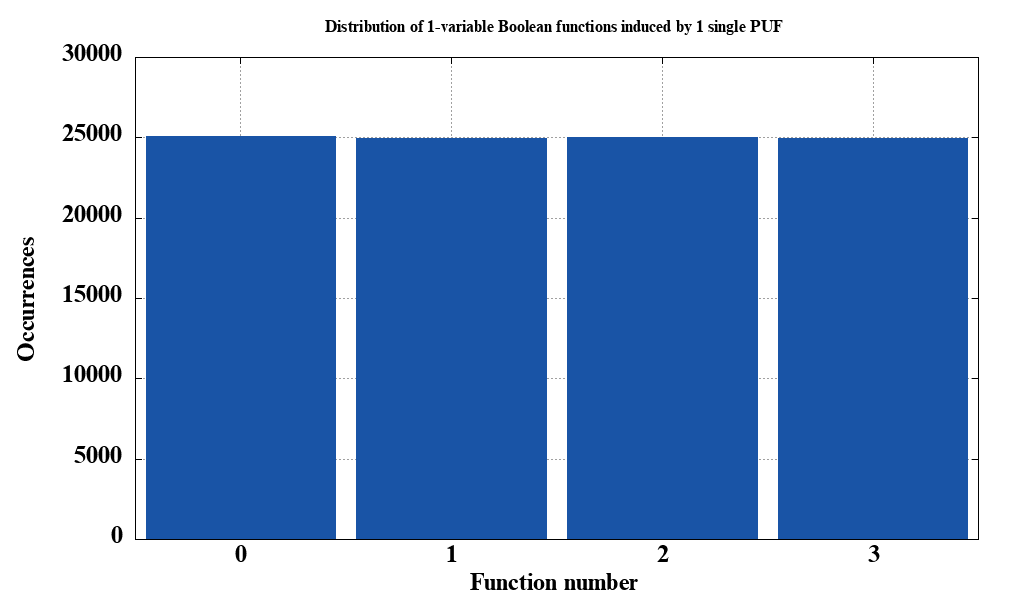
\includegraphics[width=\textwidth]{figures/dist/distribution_of_1-variable_boolean_functions_induced_by_1_single_puf.png}
    \end{figure}
\end{frame}

\begin{frame}{single arbiter puf}
    \begin{figure}
        \centering
        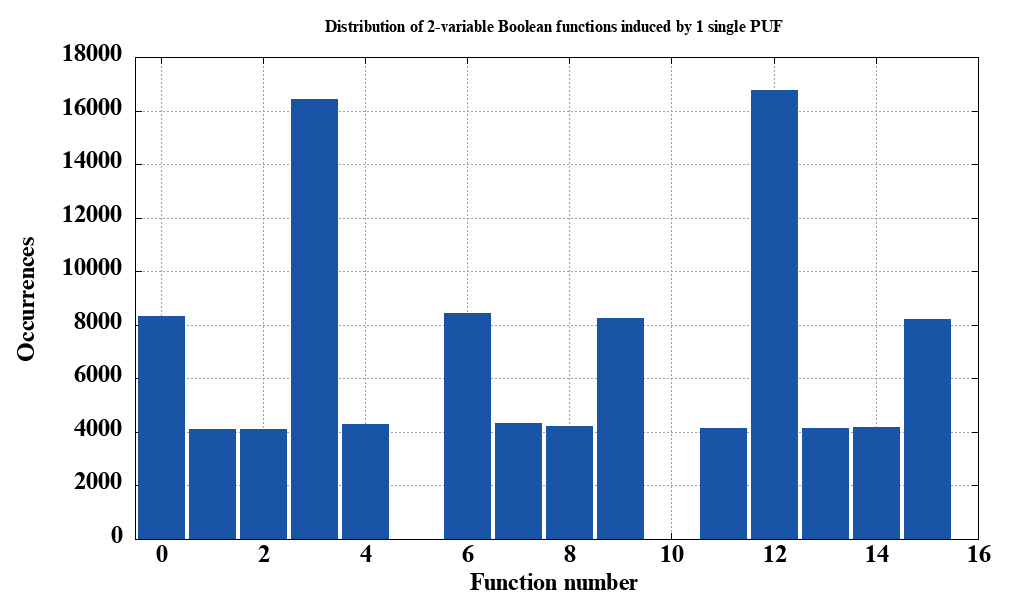
\includegraphics[width=\textwidth]{figures/dist/distribution_of_2-variable_boolean_functions_induced_by_1_single_puf.png}
    \end{figure}
\end{frame}

\begin{frame}{single arbiter puf}
    \begin{figure}
        \centering
        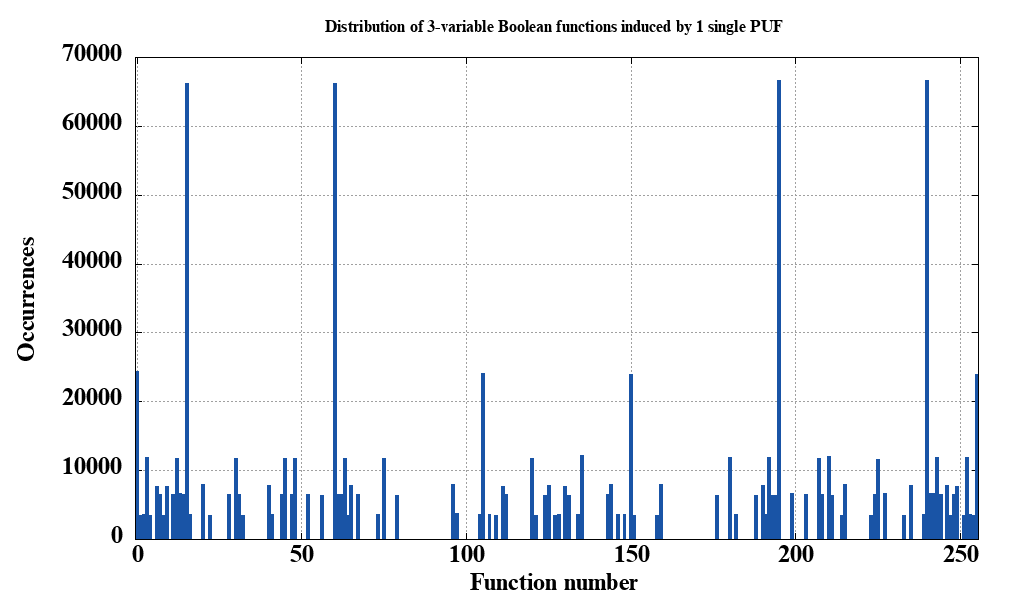
\includegraphics[width=\textwidth]{figures/dist/distribution_of_3-variable_boolean_functions_induced_by_1_single_puf.png}
    \end{figure}
\end{frame}

\begin{frame}{single arbiter puf}
    \begin{figure}
        \centering
        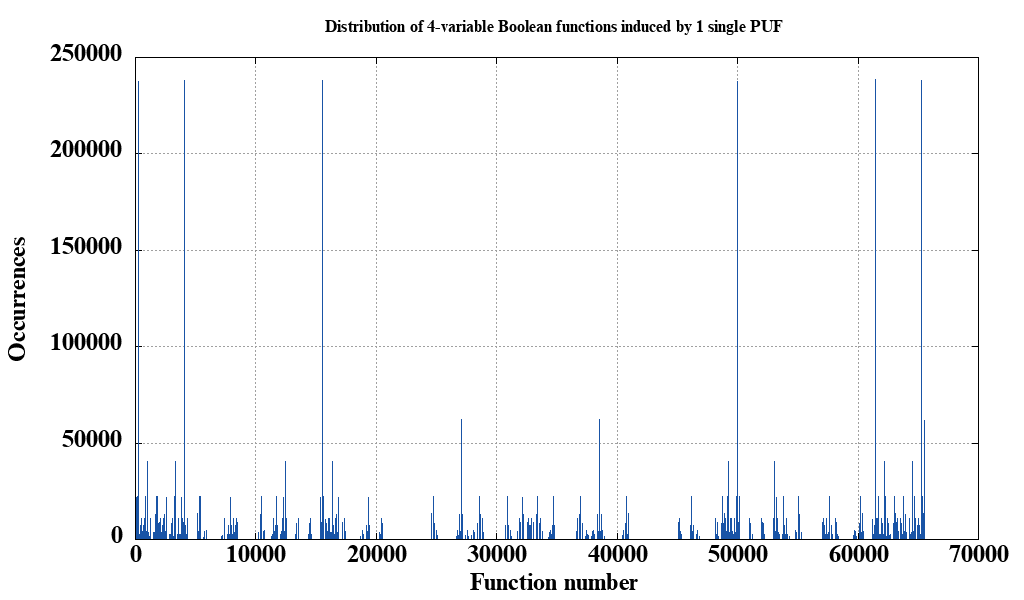
\includegraphics[width=\textwidth]{figures/dist/distribution_of_4-variable_boolean_functions_induced_by_1_single_puf.png}
    \end{figure}
\end{frame}

% --------------
% TWO PUFs XORed
% --------------

\begin{frame}{results}
    \begin{figure}
        \centering
        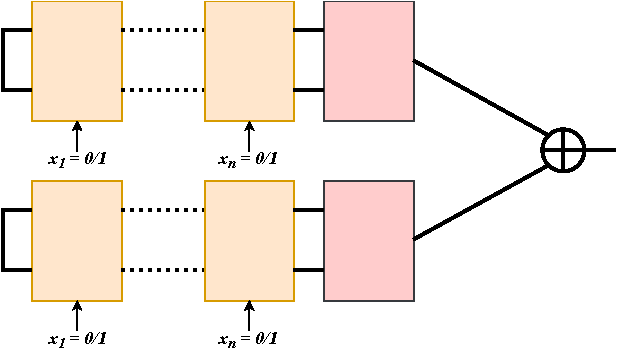
\includegraphics[width=0.7\textwidth]{figures/puf_2_xor.pdf}
        \caption{Two XORed PUFs}
    \end{figure}
\end{frame}

\begin{frame}{two xored pufs}
    \begin{figure}
        \centering
        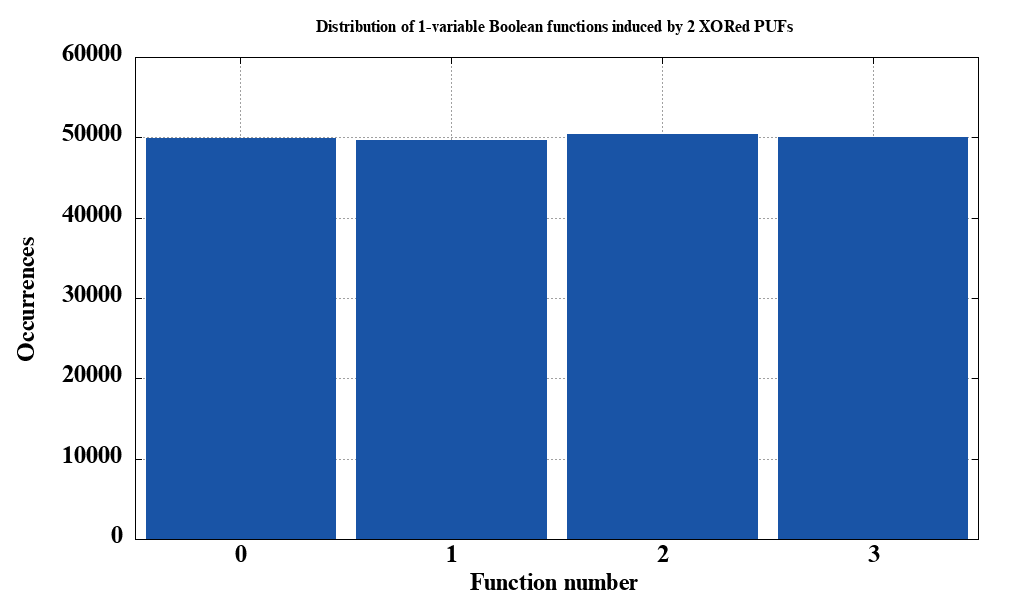
\includegraphics[width=\textwidth]{figures/dist/distribution_of_1-variable_boolean_functions_induced_by_2_xored_pufs.png}
    \end{figure}
\end{frame}

\begin{frame}{two xored pufs}
    \begin{figure}
        \centering
        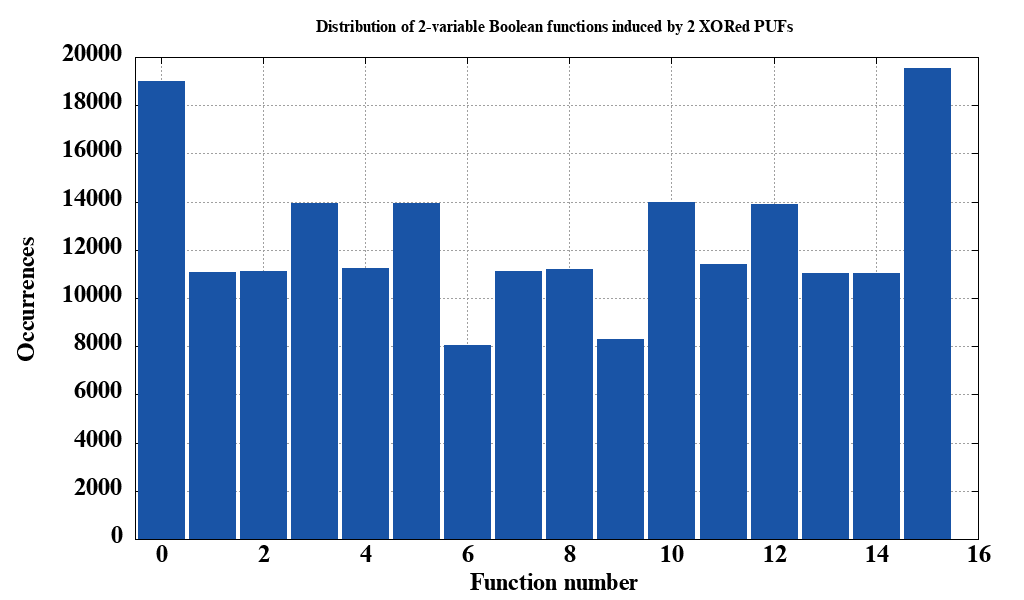
\includegraphics[width=\textwidth]{figures/dist/distribution_of_2-variable_boolean_functions_induced_by_2_xored_pufs.png}
    \end{figure}
\end{frame}

\begin{frame}{two xored pufs}
    \begin{figure}
        \centering
        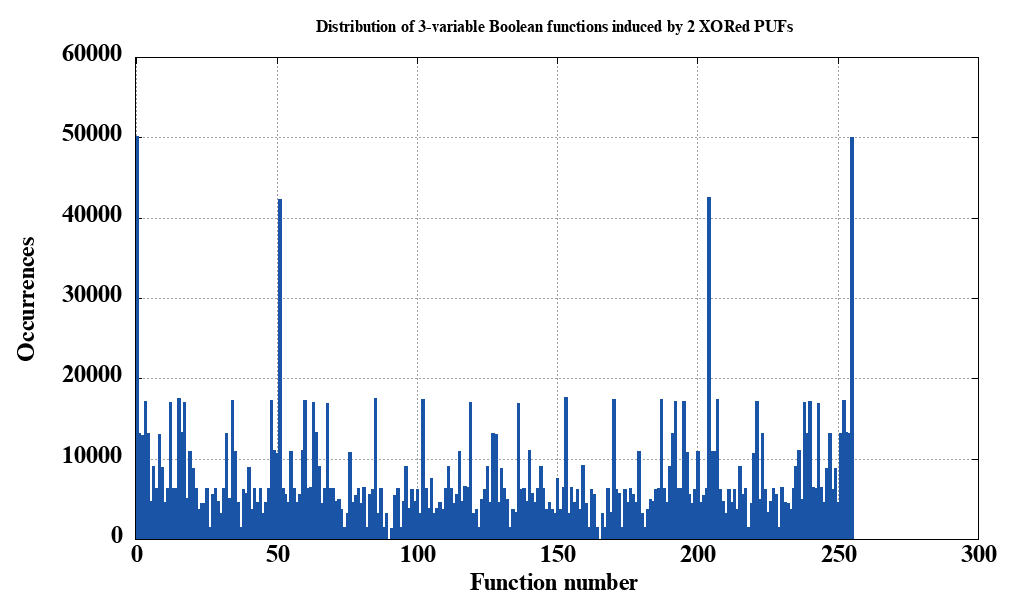
\includegraphics[width=\textwidth]{figures/dist/distribution_of_3-variable_boolean_functions_induced_by_2_xored_pufs.png}
    \end{figure}
\end{frame}

\begin{frame}{two xored pufs}
    \begin{figure}
        \centering
        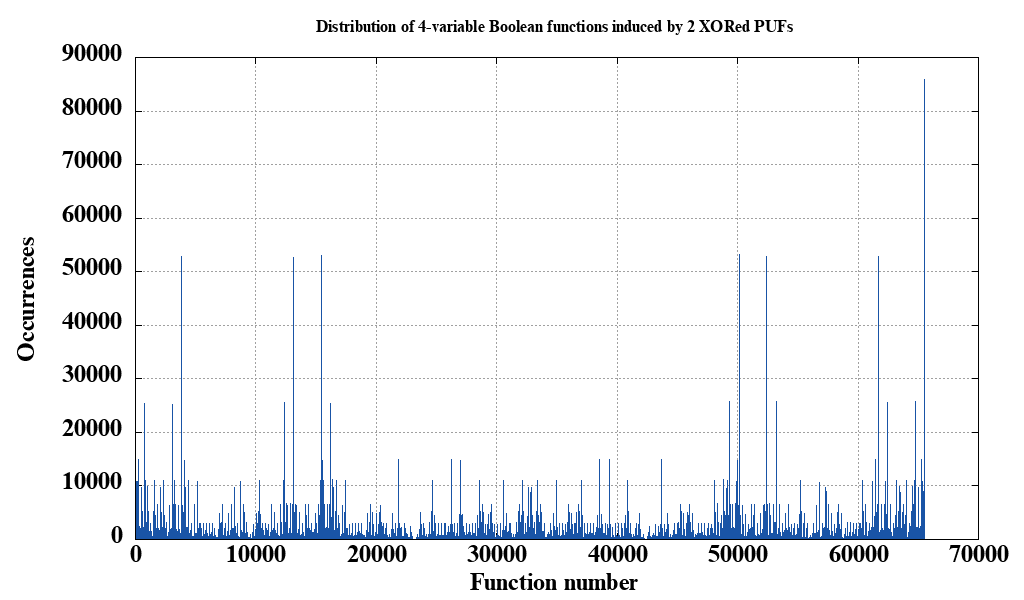
\includegraphics[width=\textwidth]{figures/dist/distribution_of_4-variable_boolean_functions_induced_by_2_xored_pufs.png}
    \end{figure}
\end{frame}

% --------------
% THREE PUFs XORed
% --------------

\begin{frame}{results}
    \begin{figure}
        \centering
        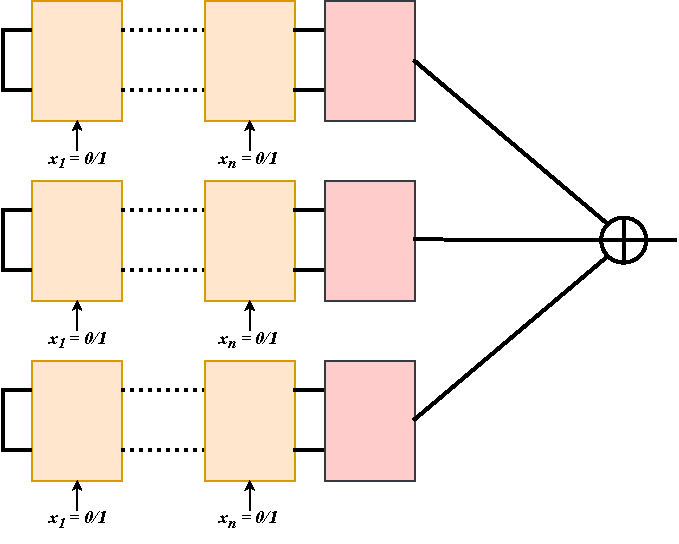
\includegraphics[width=0.7\textwidth]{figures/puf_3_xor.pdf}
        \caption{Three XORed PUFs}
    \end{figure}
\end{frame}

\begin{frame}{three xored pufs}
    \begin{figure}
        \centering
        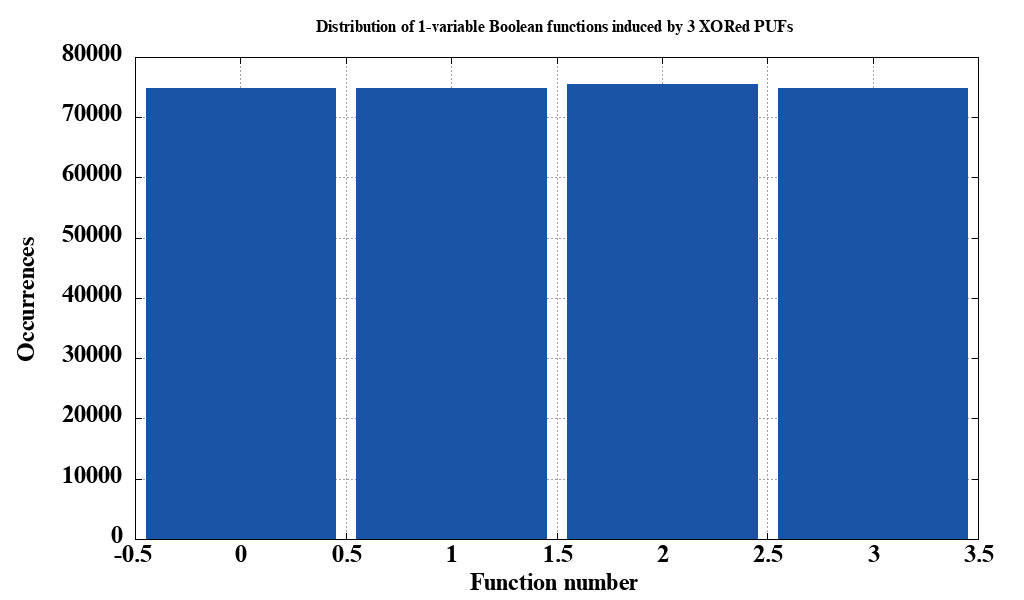
\includegraphics[width=\textwidth]{figures/dist/distribution_of_1-variable_boolean_functions_induced_by_3_xored_pufs.png}
    \end{figure}
\end{frame}

\begin{frame}{three xored pufs}
    \begin{figure}
        \centering
        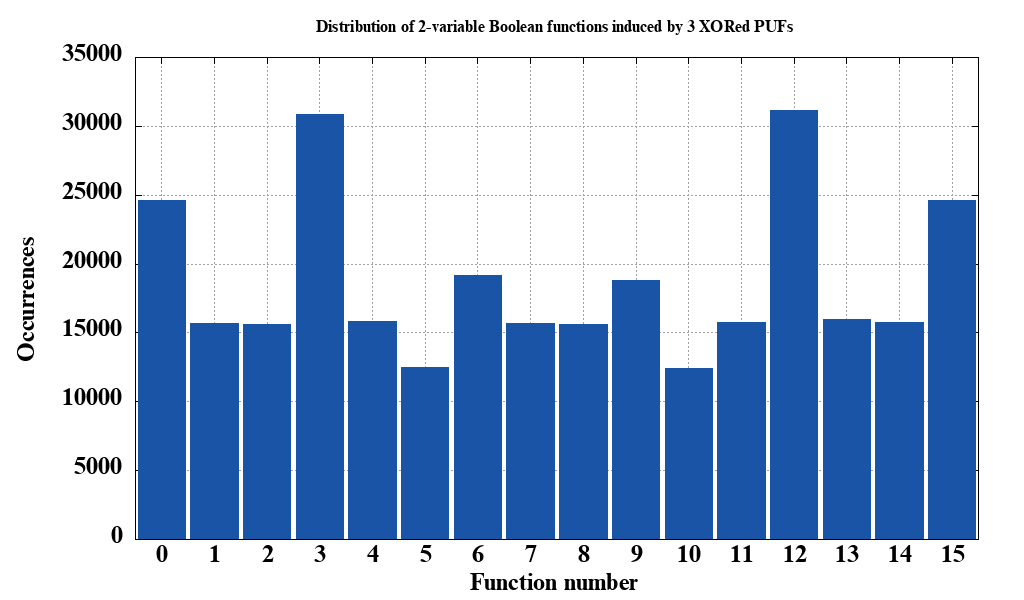
\includegraphics[width=\textwidth]{figures/dist/distribution_of_2-variable_boolean_functions_induced_by_3_xored_pufs.png}
    \end{figure}
\end{frame}

\begin{frame}{three xored pufs}
    \begin{figure}
        \centering
        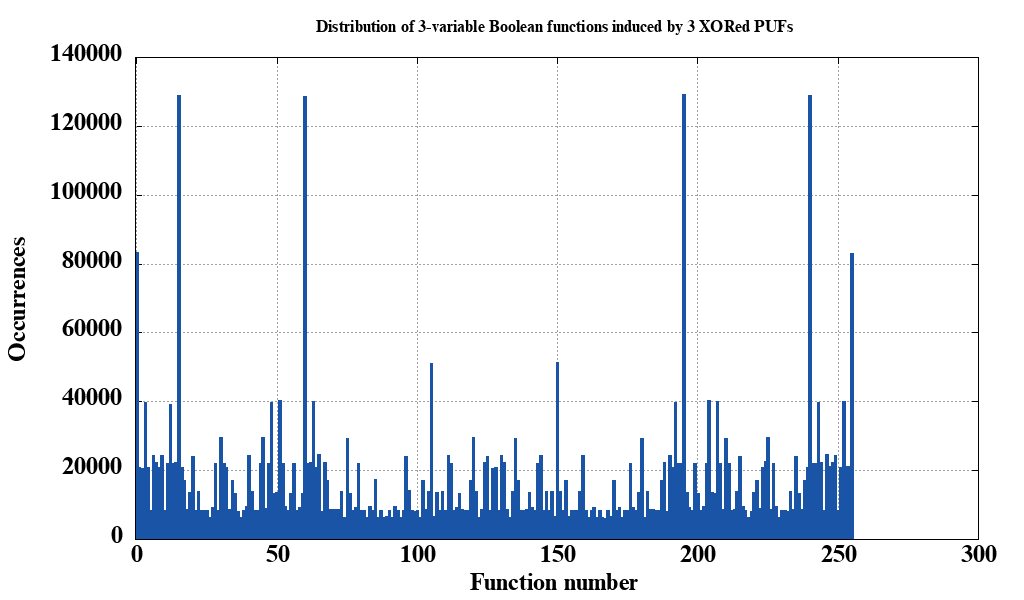
\includegraphics[width=\textwidth]{figures/dist/distribution_of_3-variable_boolean_functions_induced_by_3_xored_pufs.png}
    \end{figure}
\end{frame}

\begin{frame}{three xored pufs}
    \begin{figure}
        \centering
        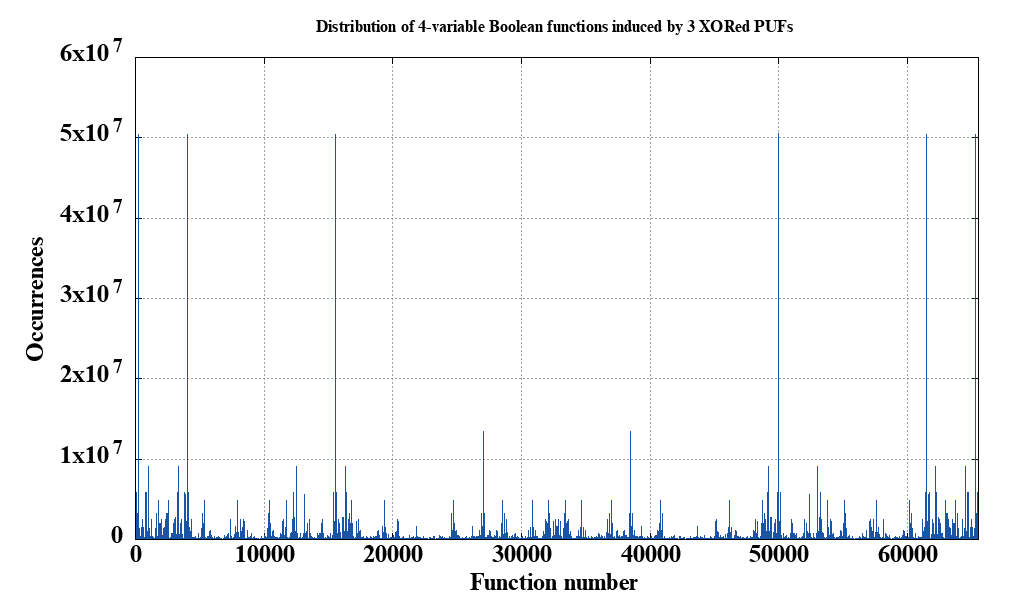
\includegraphics[width=\textwidth]{figures/dist/distribution_of_4-variable_boolean_functions_induced_by_3_xored_pufs.png}
    \end{figure}
\end{frame}

\section{summary}

\begin{frame}{summary}
    \begin{figure}
        \centering
        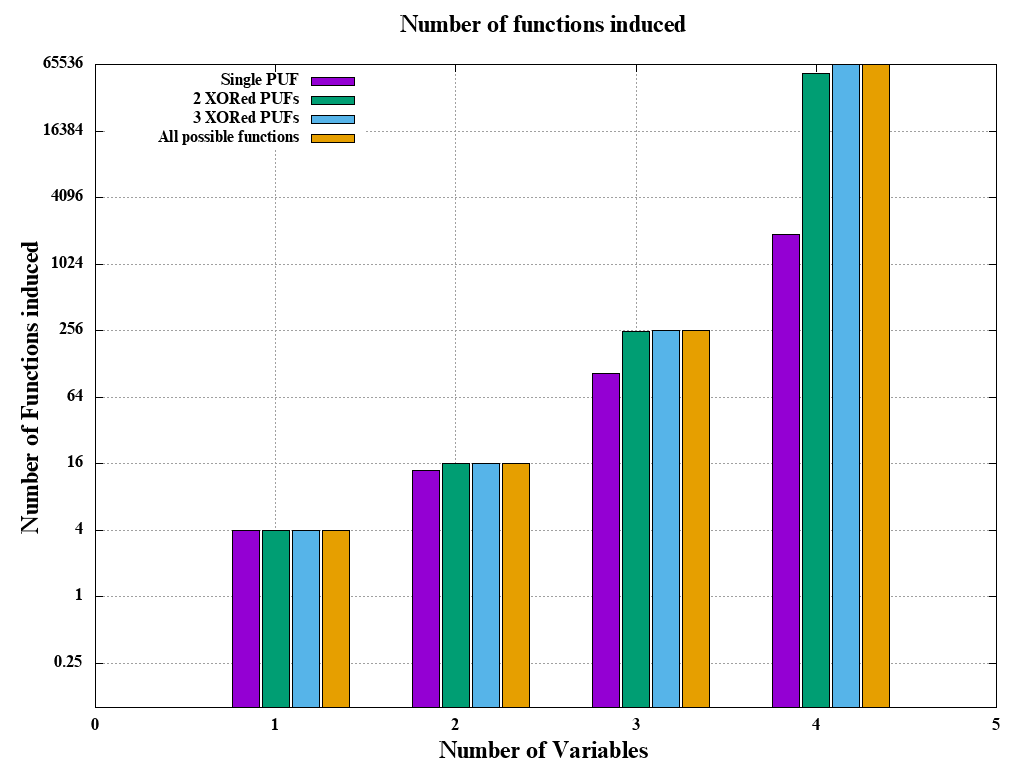
\includegraphics[width=0.9\textwidth]{figures/hist.png}
    \end{figure}
\end{frame}



\begin{frame}{overview}

    \begin{table}[H]
    \caption{Function Overview}
    \label{function_overview}    
    \def\arraystretch{1.45}
        \begin{subtable}{0.40\textwidth}
            \centering
            \begin{tabular}{|c|c|c|}
            \hline
            $n$     & $N$       & $I$                       \\ \Xhline{5\arrayrulewidth}
            1       & 4         & 0                         \\ \hline
            2       & 16        & 2                         \\ \hline
            3       & 256       & 152                       \\ \hline
            4       & 65,536    & 63,654                    \\ \hline
            \vdots  & \vdots    & \vdots                    \\ \hline
            $n$     & ${2^2}^n$ & $\geq	{2^2}^{n-1} - 2$    \\ \hline
            \end{tabular}
        \caption{One single PUF}
        \end{subtable}
        ~ 
        \begin{subtable}{0.28\textwidth}
            \centering
            \begin{tabular}{|c|c|}
            \hline
            $N$       & $I$       \\ \Xhline{5\arrayrulewidth}
            4         & 0         \\ \hline
            16        & 0         \\ \hline
            256       & 2         \\ \hline
            65,536    & 11,352    \\ \hline
            \vdots    & \vdots    \\ \hline
            ${2^2}^n$ & ???       \\ \hline
            \end{tabular}
        \caption{2 XORed PUFs}
        \end{subtable}
        ~
        \begin{subtable}{0.23\textwidth}
            \centering
            \begin{tabular}{|c|c|}
            \hline
            $N$       & $I$       \\ \Xhline{5\arrayrulewidth}
            4         & 0         \\ \hline
            16        & 0         \\ \hline
            256       & 0         \\ \hline
            65,536    & 2         \\ \hline
            \vdots    & \vdots    \\ \hline
            ${2^2}^n$ & ???       \\ \hline
            \end{tabular}
            \caption{3 XORed PUFs}
        \end{subtable}
    \end{table}
\end{frame}


\begin{frame}{Frame Title}
    \begin{table}[H]
        \centering
        \begin{tabular}{r l}
             $f(x_1,x_2) =  \begin{cases} 
                                    \overline{x_1}\\ 
                                    x_1
                                \end{cases}$ &  for $n=2$ using 1 single PUF \\
                                &\\
             $f(x_1,x_2,x_3) =  \begin{cases} 
                                    \overline{x_1 \xor x_2}\\ 
                                    x_1 \xor x_2
                                \end{cases}$ & for $n = 3$ using 2 XORed PUFs \\
                                &\\
             $f(x_1,x_2,x_3,x_4) =  \begin{cases} 
                                    \overline{x_1 \xor x_3}\\ 
                                    x_1 \xor x_3
                                \end{cases}$ & for $n = 4$ using 3 XORed PUFs
                                
        \end{tabular}
    \end{table}  
\end{frame}


\begin{frame}{hypothesis}
    \begin{center}
        $n$ XORed arbiter PUFs are needed in order to induce all ${2^2}^n$\\$n$-variable Boolean functions.
    \end{center}
\end{frame}




\begin{frame}{hypothesis}
    \begin{figure}
        \centering
        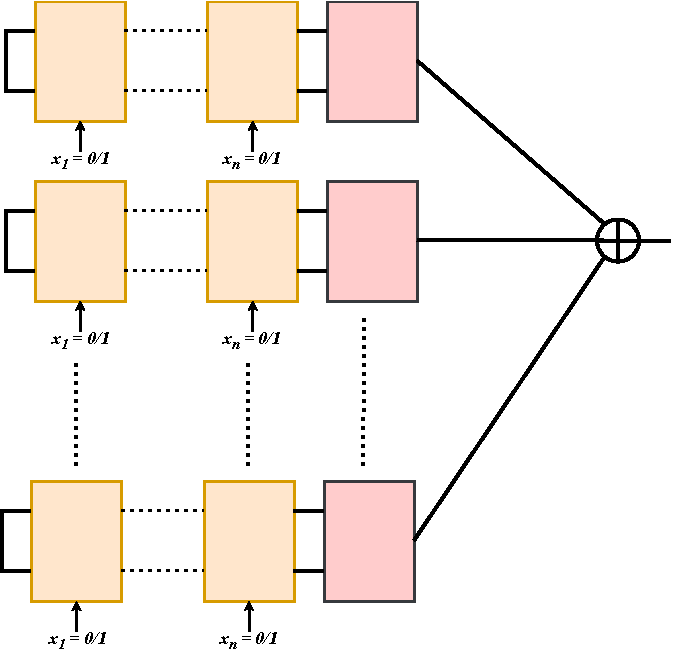
\includegraphics[width=0.6\textwidth]{figures/puf_n_xor.pdf}
        \caption{$n$ XORed PUFs to induce all possible $n$-variable functions}
    \end{figure}
\end{frame}

\section{conclusion}

\begin{frame}{future work}
    \begin{figure}
        \centering
        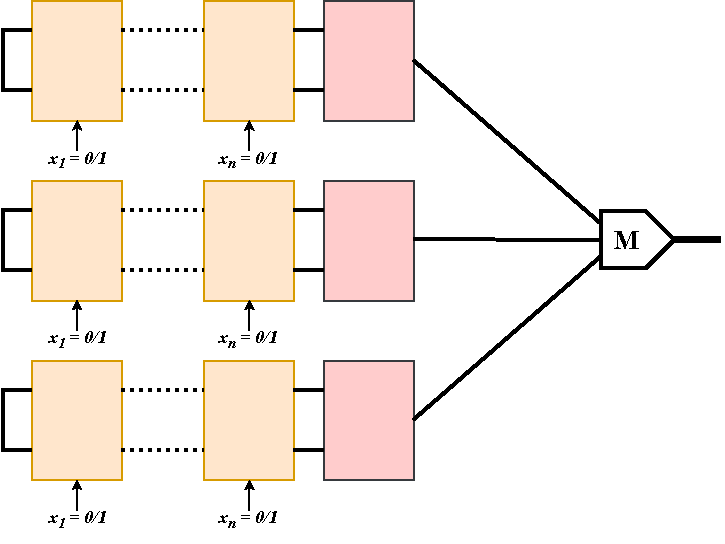
\includegraphics[width=0.6\textwidth]{figures/puf_3_maj.pdf}
        \caption{Three arbiter PUFs MAJed}
    \end{figure}
\end{frame}

\begin{frame}{acknowledgements}

    Latex Beamer:

    \begin{center}\url{github.com/matze/mtheme}\end{center}

    Graphics:
    
    \begin{center}\url{draw.io}\end{center}
    
\end{frame}


\begin{frame}{acknowledgements}
    \begin{center}
        \begin{tabular}{r l}
            Examiner: & Prof. Dr. Elena Dubrova\\
            & \\
            Mentor: & Dr. Felipe Marranghello
        \end{tabular}
    \end{center}
\end{frame}

\plain{}{Questions?}

\end{document}